% This file was created with tikzplotlib v0.10.1.
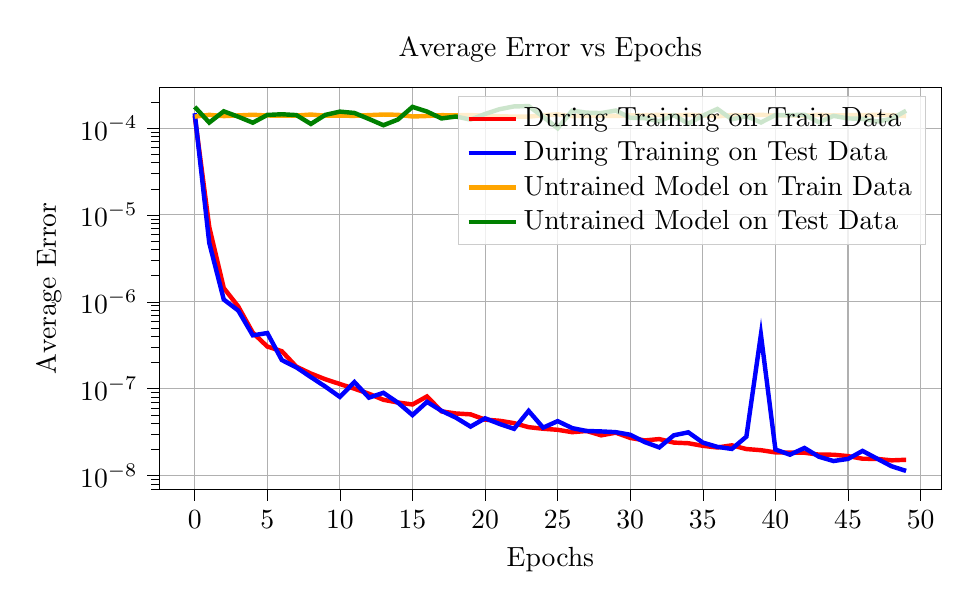
\begin{tikzpicture}

    \definecolor{darkgray176}{RGB}{176,176,176}
    \definecolor{green}{RGB}{0,128,0}
    \definecolor{lightgray204}{RGB}{204,204,204}
    \definecolor{orange}{RGB}{255,165,0}
    
    \begin{axis}[
        width = 0.95\textwidth,
        height = 19em,
    legend cell align={left},
    legend style={
      fill opacity=0.8,
      draw opacity=1,
      text opacity=1,
    %   at={(0.5,0.5)},
    %   anchor=center,
      draw=lightgray204
    },
    % log basis y={10},
    tick align=outside,
    tick pos=left,
    title={Average Error vs Epochs},
    x grid style={darkgray176},
    xlabel={Epochs},
    xmajorgrids,
    xmin=-2.45, xmax=51.45,
    xtick style={color=black},
    y grid style={darkgray176},
    ylabel={Average Error},
    ymajorgrids,
    ymin=6.96321187378274e-09, ymax=0.000290354904410608,
    ymode=log,
    ytick style={color=black},
    ytick={1e-10,1e-09,1e-08,1e-07,1e-06,1e-05,0.0001,0.001,0.01},
    yticklabels={
      \(\displaystyle {10^{-10}}\),
      \(\displaystyle {10^{-9}}\),
      \(\displaystyle {10^{-8}}\),
      \(\displaystyle {10^{-7}}\),
      \(\displaystyle {10^{-6}}\),
      \(\displaystyle {10^{-5}}\),
      \(\displaystyle {10^{-4}}\),
      \(\displaystyle {10^{-3}}\),
      \(\displaystyle {10^{-2}}\)
    }
    ]
    \addplot [ultra thick, red]
    table {%
    0 0.000138899733428843
    1 7.26432836017921e-06
    2 1.44128989632009e-06
    3 8.82225094755995e-07
    4 4.4099317619839e-07
    5 3.05433417224776e-07
    6 2.6985495082954e-07
    7 1.79246782749942e-07
    8 1.49264380411296e-07
    9 1.28192979786945e-07
    10 1.13041885185794e-07
    11 9.98787328398976e-08
    12 8.73495338282737e-08
    13 7.44121209095283e-08
    14 6.92524650958148e-08
    15 6.57125269754033e-08
    16 8.13764842177989e-08
    17 5.47648397741796e-08
    18 5.17549807454998e-08
    19 5.06033721592303e-08
    20 4.39799201501501e-08
    21 4.26815560672367e-08
    22 4.00799038402511e-08
    23 3.60131551246923e-08
    24 3.45376491850402e-08
    25 3.35878418411539e-08
    26 3.15419796947936e-08
    27 3.25466764650173e-08
    28 2.90125079516201e-08
    29 3.11344905412625e-08
    30 2.70826809867231e-08
    31 2.53443790398933e-08
    32 2.6274593167841e-08
    33 2.39348345587587e-08
    34 2.35225705580433e-08
    35 2.19639648690872e-08
    36 2.10294555103019e-08
    37 2.22524789705858e-08
    38 2.01735375071621e-08
    39 1.95676985725868e-08
    40 1.84541022463236e-08
    41 1.83214634574824e-08
    42 1.82840071971668e-08
    43 1.73900591704523e-08
    44 1.73470766640094e-08
    45 1.67271281270587e-08
    46 1.56075810053835e-08
    47 1.55275490243412e-08
    48 1.49438257324164e-08
    49 1.51756438526718e-08
    };
    \addlegendentry{During Training on Train Data}
    \addplot [ultra thick, blue]
    table {%
    0 0.00014844533870928
    1 4.76674267702037e-06
    2 1.0628197060214e-06
    3 7.92268110672012e-07
    4 4.11031038538567e-07
    5 4.36832323202907e-07
    6 2.13414253380506e-07
    7 1.75729226725707e-07
    8 1.35837808556971e-07
    9 1.0546255424515e-07
    10 8.0311629346852e-08
    11 1.19002564247239e-07
    12 7.88221186098781e-08
    13 8.94856313493619e-08
    14 6.89524028985034e-08
    15 4.96274097372407e-08
    16 7.04482232549708e-08
    17 5.55252590572763e-08
    18 4.62508005227846e-08
    19 3.654967173361e-08
    20 4.55651267827761e-08
    21 3.92327486054e-08
    22 3.44960220388657e-08
    23 5.54300179089751e-08
    24 3.55577576272026e-08
    25 4.22732249205637e-08
    26 3.51410207599656e-08
    27 3.25441220638822e-08
    28 3.21748352405393e-08
    29 3.15483639212744e-08
    30 2.94743696116484e-08
    31 2.42509656800394e-08
    32 2.1060678534468e-08
    33 2.90387500712086e-08
    34 3.14091828101937e-08
    35 2.39285675718293e-08
    36 2.13697148865322e-08
    37 2.02332923748827e-08
    38 2.80337761893179e-08
    39 4.1882645973601e-07
    40 1.9922834937347e-08
    41 1.73602039410525e-08
    42 2.07416608333233e-08
    43 1.64387952139577e-08
    44 1.46818992519115e-08
    45 1.55218575770277e-08
    46 1.92011722077723e-08
    47 1.56486414937262e-08
    48 1.27744943512198e-08
    49 1.12931486384582e-08
    };
    \addlegendentry{During Training on Test Data}
    \addplot [ultra thick, orange]
    table {%
    0 0.000135580819915049
    1 0.000142116216011345
    2 0.000137380717205815
    3 0.000139936193590984
    4 0.000142444492666982
    5 0.000139559400849976
    6 0.000139205061714165
    7 0.000139498966746032
    8 0.000143201788887382
    9 0.000139012030558661
    10 0.000138873860123567
    11 0.000138410890940577
    12 0.00014102082059253
    13 0.000143270721309818
    14 0.000142237113323063
    15 0.000135978290927596
    16 0.000137778275529854
    17 0.00014073250349611
    18 0.000140512682264671
    19 0.000141123935463838
    20 0.00013889440742787
    21 0.000137015958898701
    22 0.00013543690147344
    23 0.000135413778480142
    24 0.000140565694891848
    25 0.000144005738548003
    26 0.000137403549160808
    27 0.00013848849630449
    28 0.000138961564516649
    29 0.00013785291230306
    30 0.000140357617055997
    31 0.000140674586873502
    32 0.000142057760967873
    33 0.000139720403240062
    34 0.000142506891279481
    35 0.000140076066600159
    36 0.000136208720505238
    37 0.000141315162181854
    38 0.000139822936034761
    39 0.000142146338475868
    40 0.000139813200803474
    41 0.000139538722578436
    42 0.000139243988087401
    43 0.000142359247547574
    44 0.000139776835567318
    45 0.000140800751978531
    46 0.000140809308504686
    47 0.000142282297019847
    48 0.000141126482049003
    49 0.000137355818878859
    };
    \addlegendentry{Untrained Model on Train Data}
    \addplot [ultra thick, green]
    table {%
    0 0.000175602370291017
    1 0.000115721581096295
    2 0.000156029564095661
    3 0.000135122318170033
    4 0.000115373361040838
    5 0.000141736381920055
    6 0.000144295612699352
    7 0.000141208045533858
    8 0.000111631678009871
    9 0.000142020973726176
    10 0.000154777924763039
    11 0.000149349492858164
    12 0.000127313614939339
    13 0.000107892628875561
    14 0.000125519931316376
    15 0.000175431167008355
    16 0.000155052868649364
    17 0.00012920267181471
    18 0.000135864058393054
    19 0.000125273712910712
    20 0.000145317215356044
    21 0.000164944241987541
    22 0.000177754482137971
    23 0.000179029142600484
    24 0.000135274472995661
    25 9.9544799013529e-05
    26 0.000158733208081685
    27 0.000150573701830581
    28 0.000148892766446806
    29 0.000159243267262354
    30 0.000131555570987985
    31 0.000129963023937307
    32 0.00011968205217272
    33 0.000140874632052146
    34 0.000112492547486909
    35 0.000139083160320297
    36 0.0001660277339397
    37 0.000126232087495737
    38 0.000137334165628999
    39 0.000116096263809595
    40 0.000141106240334921
    41 0.000140998396091163
    42 0.000142489516292699
    43 0.000116595139843412
    44 0.000138309842441231
    45 0.000129201245727018
    46 0.000127760227769613
    47 0.000119176627777051
    48 0.00012781129044015
    49 0.000158458482474089
    };
    \addlegendentry{Untrained Model on Test Data}
    \end{axis}
    
    \end{tikzpicture}
    